\documentclass[a4paper]{article}

%% Language and font encodings
\usepackage[english]{babel}
\usepackage[utf8x]{inputenc}
\usepackage[T1]{fontenc}
\usepackage{float}
\usepackage{tikz}
\usetikzlibrary{matrix}
\usepackage{algpseudocode} 

%% Sets page size and margins
\usepackage[a4paper,top=3cm,bottom=2cm,left=3cm,right=3cm,marginparwidth=1.75cm]{geometry}
\usepackage{amsmath}
\usepackage{amsthm}
\usepackage{amssymb}

\newtheorem{theorem}{Theorem}
\newtheorem{lemma}[theorem]{Lemma}

\begin{document}
\section*{External memory mergesort}
In the external-memory model (hereafter EM model),
show how to implement the k-way merge (where $(k + 1)B \leq M$), namely, how to
simultaneously merge k sorted sequences of total length N, with an I/O cost of $O(N/B)$
where B is the block transfer size. Also, try to minimize and analyze the CPU time
cost.
\\
\\
\textbf{SOLUTION}
\\
\\
The classical external sorting algorithm, called merge-sort, consists of two phases:
\begin{enumerate}
\item \textbf{The sort phase}. B element are read into the buffer, sorted, and written to the
disk. This creates $n =\lceil N/B \rceil$ sorted subset of records, called runs, stored
in separate auxiliary files, numbered from 1 to n. The runs have all the same
number of pages, B, except the last.
\item \textbf{The merge phase} consists of multiple merge passes. In each merge pass, $k = B−1$
runs are merged using the remaining buffer page for output. At the end of a merge
pass, the number of runs becomes $n=\lceil n/k \rceil$. A merge pass is repeated until
n > 1. The merge is done transferring k blocks in main memory from the $n$, keeping the minimum from each run, and store it in another block (notice is the reason for k+1 block). When we full fill the latter block we transfer it in external memory.   
\end{enumerate}
This is possible because $(k + 1)B \leq M$.
\begin{figure}[H]
\centering
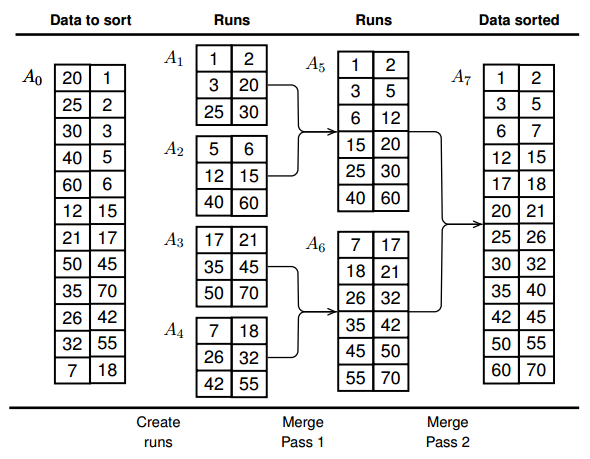
\includegraphics[scale=0.4]{kway.png}
\caption{Let us show how to sort the file $A_0$ containing 12 pages, with file and buffer pages
capacity of 2 records[\textbf{IT'S AN EXAMPLE} no need to consider the records], B = 3 and 2-merge passes.}
\end{figure}
\begin{itemize}
\item The initial sort phase creates the runs $A_1$, $A_2$, $A_3$ and $A_4$.
\item The first merge pass creates the runs $A_5$ and $A_6$ by merging $A_1$, $A_2$ and $A_3$,$A_4$.
\item The second merge pass creates the sorted data $A_7$ by merging $A_5$, $A_6$.
\end{itemize}
At each iteration of merge we read $\lceil N/B \rceil$ block and the same for the writing. Therefore we have $O(N/B)$ I/O operation.
\\
\\
The bottle neck in CPU cost is to search of the min key in the k runs each time we add an element in the output block. Indeed if we do a linear search we pay $O(k)$ at each element, then a total of $O(Nk)$. Instead, if we use an MinHeap (priority queue), we pay $O(log \ k)$ to insert an element in the Heap and O(1) to retrieve the min. Therefore the total cost in $O(N log \ k)$. 
\end{document}